\section{Mumuki: An online coding tool} \label{the-approach}

%length: 1 page
%resposible: Fede & Franco

%content:
%general descrition of Mumuki
%description and example of test cases and expectations

Mumuki is a free and open source\footnote{Source code available at \url{https://github.com/mumuki}.} web-based coding tool that provides automatic formative feedback and assessment, developed in Argentina. This platform provides assistance for teachers and students, in a process conducted by practice where theory arises from the exercises. It supports several programming languages: Haskell, Prolog, Python, JavaScript and C. Mumuki is currently used at six Argentinian universities, five high schools and two coding clubs\footnote{The complete list of organizations using Mumuki can be found at \url{http://www.mumuki.org} (in Spanish).}, with more than 1500 active users.

Practice within the platform is organised across topics with many programming exercises\footnote{The exercises are available at \url{http://mumuki.io}} each. An exercise includes two 
parts. On the one hand, it includes a description of the problem the student should solve by providing a program, in which generally, no more than a few functions are required. On the other hand, the exercise designer provides a way to automatically compute feedback for the solution of the exercise at two different levels: correctness and quality. For correctness, a suite of representative unit tests are provided by the teacher and executed against the final program. The final program could include auxiliary functions  programmed by the teacher. Although correctness cannot be assured by this technique, it proved to be good enough for the complexity  of the existent exercises. Regarding the quality of the student solution, the abstract syntax tree is used. By using an editor tool, the teacher can pick several predefined patterns, called \emph{expectations} in Mumuki. Expectations are defined so that
they must be present or not present in the student’s solution. When the student submits a solution, each expectation is evaluated against it.

%The teacher defines a set of regular expressions, called \emph{expectations} in Mumuki, specifying patterns that should be present in the student's solution. When the student submits a solution, each expectation is evaluated against it.

Imagine the following scenario. When explaining lists, the teacher wants to write an exercise to introduce the \hs{filter} function. This exercise asks the student to define a function called \hs{onlyEvenNumbers} that returns only the even numbers of a given list. The exercise description is illustrated by the example \hs{onlyEvenNumbers [8,7,6,5] = [8,6]}. 
The following unit tests are provided by the exercise designer and not shown to the student until he submits a solution.
\begin{itemize}[noitemsep,topsep=0pt]
    \item {Expect \hs{onlyEvenNumbers [] = []}.}
    \item {Expect \hs{onlyEvenNumbers [1,2,3] = [2]}.}
    \item {Expect \hs{onlyEvenNumbers [7,14,9,10] = [14,10]}.}
\end{itemize}

The teacher also defines the following expectations. Because the use of \hs{filter} is expected, direct recursion is not allowed. This is specified by the teacher as a pattern that \emph{should not} be found in the student solution. Also, the teacher wants to encourage code reuse, so the solution must use the \hs{even} function provided by Haskell's standard libraries. This is specified by the teacher as a pattern that \emph{should} be found in the student solution. 
%Summing up, the exercise expectations are the following.
%\begin{itemize}[noitemsep,topsep=0pt]
%    \item {\hs{onlyEvenNumbers} should not use direct recursion.}
%    \item {\hs{onlyEvenNumbers} should use \hs{even}.}
%\end{itemize}

In Figure~\ref{fig:recursion} the student uses \hs{even} but she uses direct recursion instead of using \hs{filter} in the solution. Mumuki informs the test results are correct but an expectation is not met. It explains that the student must not use recursion. The exercise is assessed by Mumuki as yellow: tests results are correct but some expectation is not met. 

In Figure~\ref{fig:error} the student did not use \hs{even} and he made a mistake when programming his version of even. Instead of verifying that the modulus operation is zero, he compares it to one. Both the tests and one of the expectations fail, and this is reported by Mumuki. The exercise is assessed by Mumuki as red because some test results are incorrect. 

\begin{figure}

%\textbf{Solution:}
\begin{minted}{haskell}
SOLUTION: onlyEvenNumbers [] = []
          onlyEvenNumbers (x:xs)
            | even x    = x:(onlyEvenNumbers xs)
            | otherwise = onlyEvenNumbers xs

FEEDBACK:
\end{minted}
%\textbf{Feedback:}\\
%\ \\
\vspace*{-0.7cm}
\hspace*{1.5cm}\mbox{
    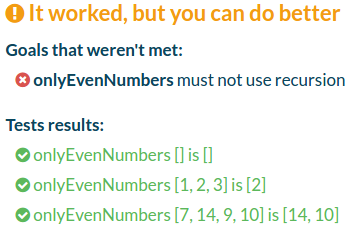
\includegraphics[width=0.32\textwidth]{screenshots/atheneum-warning-direct-recursion-used.png}
    }
    
\caption{Sample solution to an exercise which is assessed as yellow by Mumuki because test results are correct but some expectation is not met.\label{fig:recursion}}

\end{figure}    

Student solutions are assessed by Mumuki with three possible values: red, yellow or green. Red indicates that some test result is not correct. Yellow means that all tests are correct but some expectation is not met. An exercise is marked green when all tests are correct and all expectations are met. 

Every solution submitted by a student is stored, thus the teacher has access not only to the final solution but also to all the steps that lead to it. The timestamp, the tests and expectations results, the result of the execution and the status that was reported to the student are also stored, so the full history can be reproduced. This information, along with the student's profile, could be useful to improve the exercises, to explore common mistakes, etc.

\begin{figure}[H]
%\textbf{Solution:}
\begin{minted}{haskell}
SOLUTION: onlyEvenNumbers ls = 
            filter (\x -> x `mod` 2 == 1) ls

FEEDBACK:
\end{minted}
    
%\textbf{Feedback:}\\
%\ \\
\vspace*{-0.7cm}
\hspace*{1.5cm}\mbox{
    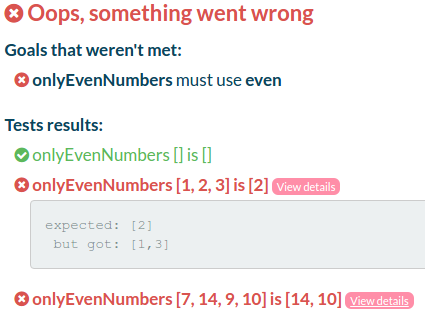
\includegraphics[width=0.4\textwidth]{screenshots/atheneum-error-tests-failed.png}
}
    
    \caption{Sample solution to an exercise that is assessed as red by Mumuki because some tests results are incorrect.\label{fig:error}}
\end{figure} 

The logged data is presented on a web page as shown in Figure~\ref{fig:classroom} and can be accessed only by the teachers. In the web interface, the teachers can monitor students' progress, view the difference between submissions and send comments to the student about particular solutions. 

Two solutions for the same exercise and their difference are reported on the teacher's tool, using a diff highlighting library that allows to visualise it in either way. Visualisation can be \emph{unified} showing line by line differences in the same panel and highlighting the differences as illustrated in Figure~\ref{fig:classroom}. Or it can be \emph{split} side by side, with two different panels showing two different submitted solutions. The figure also shows the textbox that the teacher can  use to send comments associated to a particular student submission. In the figure, the student has submitted ten different solutions for this exercise. The last one is marked green by Mumuki since it passes all the tests and meets all the expectations. 

\begin{figure}
    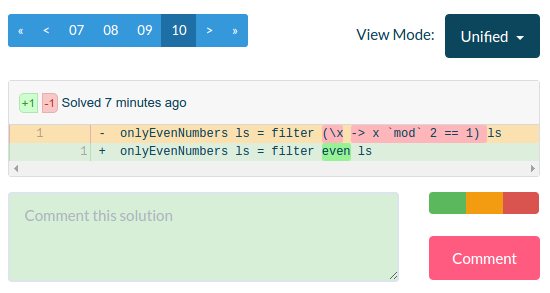
\includegraphics[width=0.46\textwidth]{screenshots/classroom-unified-diff.png}
    
    \caption{Two solutions for the same exercise and their difference are reported on the teacher's tool, using a diff highlighting tool.}
    \label{fig:classroom}
\end{figure}
